\chapter{Storage ring setup, diagnostics, measurements \& experimental methods}
In this chapter, we delve into the SIRIUS magnetic lattice, beam diagnostics tools and relevant experimental methods. We emphasize the key parameters  for optimizing nonlinear dynamics and detail the experimental procedures encompassing beam trajectories and orbits, beam current and lifetime, as well as the control and manipulation of tunes and chromaticity during machine studies. The final segments address the selection of objective functions for probing the Dynamic Aperture and the selection of sextupole families as optimization knobs.

\section{SIRIUS magnetic lattice}
\label{sec:mag_latt}
SIRIUS storage ring consists on a 20-cell five-bend-achromat (5BA) lattice comprising a 5-fold symmetric configuration with alternating high and low horizontal betatron functions at the straight sections, as Fig.~\ref{fig:5BA_lattice} shows. There are 5 A-type sections, with high horizontal betatron function and 15 B- and P-type sections, with low horizontal and vertical betatron functions \cite{liu_new_2016}.
% While the B and P sections share identical linear lattice elements (dipoles and quadrupoles\footnote{The quadrupole families are in fact distinct. Their strengths can be changed and this symmetry can be broken. Currently the strengths of the quadrupoles in the B and P sections are the same.}), they differ in their sextupoles.
A superperiod consists of one high-beta and 3 low-beta sections arranged in the order A-B-P-B.
% Among the 20 straight sections, 17 are allocated for insertion devices (IDs), 2 for machine installations, and 1 for shared use between a small ID and machine installation [21].

The central dipole, the BC, is a permanent superbend magnet with a peak field of $3.2~\unit{T}$. The storage ring accommodates 20 such. The arcs contain additional four dipoles: two B1 and two B2. These are electromagnetic dipoles with peak fields of $0.58~\unit{T}$. In total, the SIRIUS magnetic lattice comprises 100 dipoles: 20 permanent BC magnets and 80 B1 and B2s electromagnets.

In the high-beta straight sections, the quadrupole doublet (QFA, QDA) is employed for optics matching. B-type sections utilize the (QFB, QDB1, QDB2) quadrupole triplet for matching while the (QFP, QDP1, QDP2) triplet is used in the P-type sections. The arc sections contain the Q1, Q2, Q3, and Q4 quadrupole families, totalling 12 families of quadrupoles and 270 magnets.

The lattice also features 21 families of sextupoles magnets, used for chromaticity correction and nonlinear dynamics optimization. They sum up to 280 magnets. Some sextupoles families are located where the dispersion function vanishes and are called \textit{achromatic}, or harmonic, while other families, located where there is non-zero dispersion, are called \textit{chromatic} families.

Table~\ref{tab:sext_fams} lists the sextupoles families and their types in the storage ring. The 21 families are, in principle, the available search space for nonlinear dynamics optimization. The subsection~\ref{subsec:knobs}, on the choice of optimization knobs, at the end of this chapter, shows how the search space can be reduced down to 13 dimensions once the constant chromaticity requirement and/or other additional constraints are imposed.

\begin{figure}[htb]
    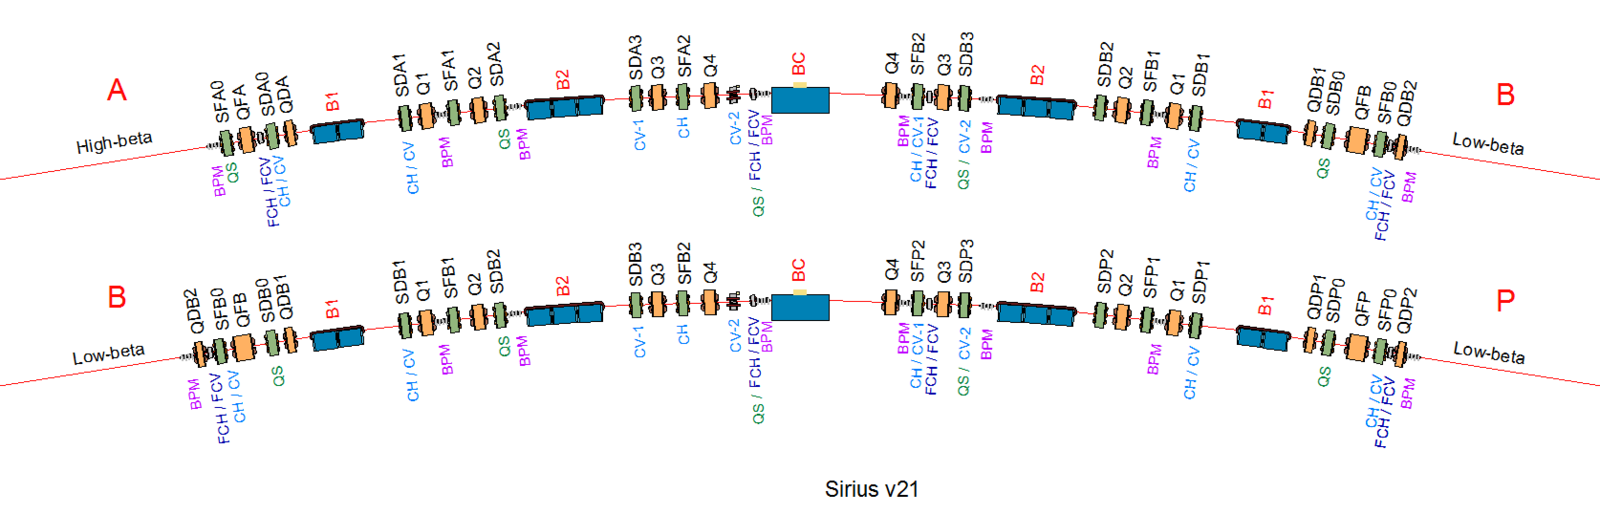
\includegraphics[width=\textwidth]{Images/sirius_arcs.png}
    \caption[SIRIUS 5BA cells comprising the lattice.]{SIRIUS 5BA cells comprising the lattice. The cells differ by their straight section types: high-beta type (A), or low-beta (B, P). A superperiod consists of one high-beta and 3 low-beta sections arranged in the order A-B-P-B. The storage ring consists on 5 concatenation of superperiods. Source: Wiki-SIRIUS (currently only available on-campus).}
    \label{fig:5BA_lattice}
\end{figure}

\begin{table}[htb]
    \caption{SIRIUS sextupole families}
    \centering
        \begin{tabular}{ll}
        \hline
        achromatic                                                                      & chromatic                                                                                                                                          \\ \hline
        \begin{tabular}[c]{@{}l@{}}SFA0, SDA0, SFB0,\\ SDB0, SDP0, SFP0\end{tabular} & \begin{tabular}[c]{@{}l@{}}SDA1, SFA1, SDA2, SFA2,SDA3, SDB1, SFB1,\\ SDB2, SFB2, SDB3, SFP1, SDP1, SDP2, SFP2, SDP3\end{tabular}
        \end{tabular}
        \label{tab:sext_fams}
\end{table}

% For coupling control and the beam-based alignment (BBA) process \cite{cruz_aplicacoes_2022} there are 5 skew quadrupoles (QS) per arc, totaling 100 QS in the storage ring. At each arc, 4 of the QS are realized as additional coils in sextupole magnets and account for coupling, while the other, immediately before the BC, is realized in a dedicated corrector magnet and required for BBA.

% Besides the lattice magnets, SIRIUS has correction dipole magnets distributed among the two types of correction systems available: fast orbit correction and slow orbit correction. Both of them share the same orbit diagnostic device probing the beam's centroid positions: beam position monitors (BPMs). Each arc section is equipped with 8 BPMs, totaling 160 BPMs in the storage ring.  For the slow orbit correction system, each section has 6 horizontal correctors (CH) and 7 vertical correctors (CV), both installed in sextupole magnets. An extra vertical corrector magnet is installed per arc, resulting in 120 CHs and 160 CVs in the storage ring.

% The fast orbit correction system comprises 4 horizontal and 4 vertical fast correctors (FCH and FCV, respectively) per sector, totaling 80 FCH and 80 FCV (2 FCH and 2 FCV per source point). The Slow Orbit Feedback system (SOFB) and the Fast Orbit Feedback (FOFB) system currently oversee the slow and fast orbit corrections simultaneously.

\section{Beam diagnostics and measurements}
\subsection{Beam positions}
To track the beam's position along the ring, a diagnostic tool known as Beam Position Monitor (BPM) employs a set of four pick-up antennas positioned within the vacuum chamber, as illustrated by Fig~\ref{fig:bpms_scheme}. The mirror charges induced by the electron beam are collected by the antennas. The determination of beam displacements relies on the differential signal induced on the antennas when the beam deviates from the device's geometric center. The induced voltage signal undergoes processing in the "partial-Delta/Sigma" scheme, providing horizontal and vertical beam displacements through the following algebraic calculations:
\begin{equation}
    x = K_x \qty[\frac{A-C}{A+C}+\frac{D - B}{D+B}], \quad y = K_y \qty[\frac{A-C}{A+C}-\frac{D - B}{D+B}],
\end{equation}
where $A$, $B$, $C$, and $D$ represent the intensity of the induced signal over the corresponding antennas. The calibration factors $K_x$ and $K_y$ are determined to correct the discrepancy between the measured values and the actual positions of the beam. 

SIRIUS is equipped with 160 BPMs distributed along the storage ring. The BPMs allow the determination of the centroid's displacements at a turn-by-turn (TbT) acquisition rate for probing the betatron motion. The signal can also be processed at other acquisition rates, allowing for signal averaging and providing information about the orbit.
\begin{figure}
    \centering
    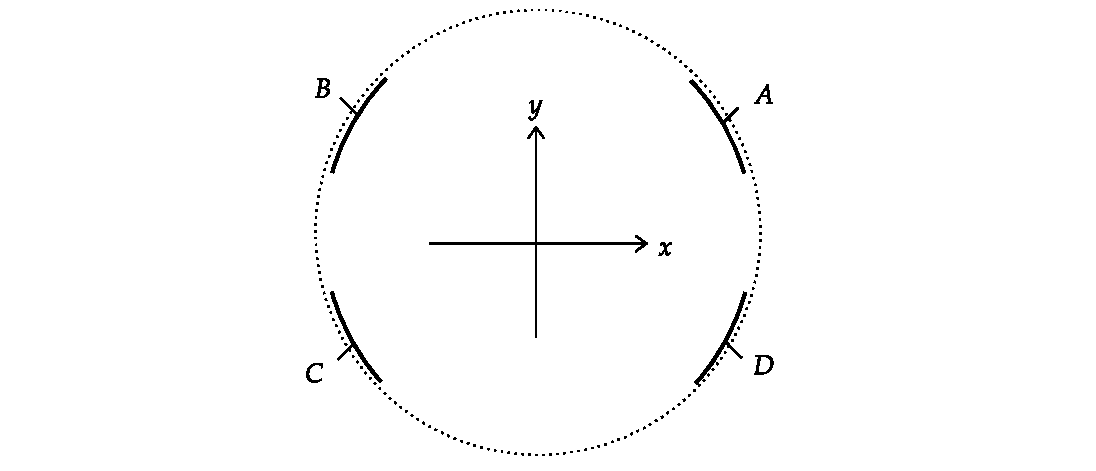
\includegraphics[width=\textwidth]{Images/bpm_scheme.pdf}
    \caption[Schematic representation of BPM button antennas, the vacuum chamber cross-section, and the transverse positions reference frame.]{Schematic representation of BPM button antennas, in solid lines, the vacuum chamber cross-section, in dashed lines, and the transverse positions reference frame.}
    \label{fig:bpms_scheme}
\end{figure}
\subsubsection{Phase-space reconstruction and decoherence}
With BPMs recording the turn-by-turn motion of the beam's centroid, the $x$ and $y$ positions can be readily acquired. The angles, or momenta, can be obtained through the following processing: for two consecutive BPMs located at the ends of a straight section of length $\ell$, where no bending or focusing occurs, the beam angle can be calculated as $x^\prime = \frac{\Delta x}{\ell}$, where $\Delta x$ refers to the difference in position readings from the BPMs. This allows for the reconstruction of the $x, x^\prime$ and $y, y^\prime$ phase-spaces on a turn-by-turn basis, as exemplified by Fig.~\ref{fig:phase_space_recons}. In the figure, BPM data of the beam was acquired at the TbT rate, soon after betatron oscillations were induced to the beam's centroid. The beam initially had an amplitude in the negative horizontal direction reaching approximately $-8~\unit{mm}$ and in the first turns it circulated the outermost region of the phase portrait (dark blue points). The last turns correspond to light yellow points in the innermost region.
\begin{figure}
    \centering
    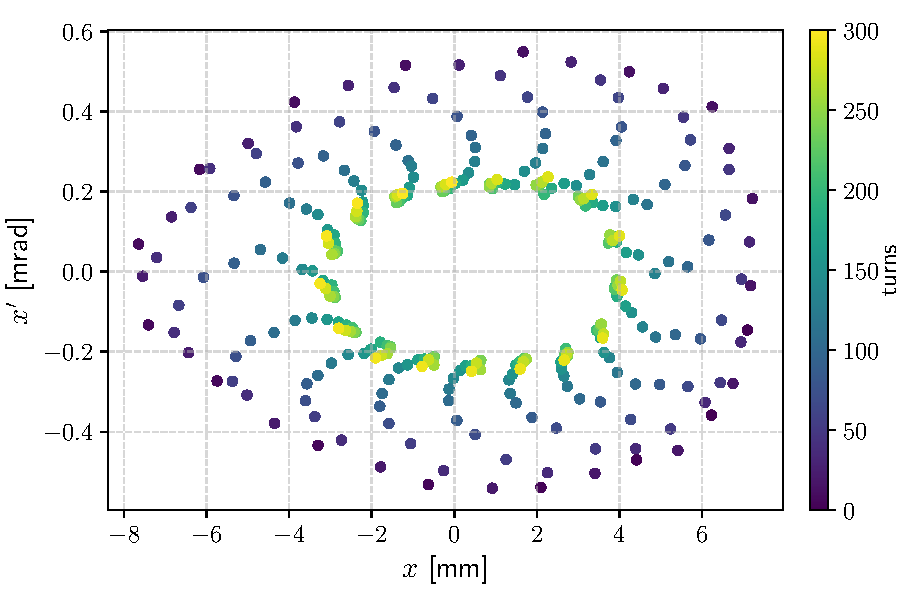
\includegraphics[width=0.7\textwidth]{Images/phase_space_recons.pdf}
    \caption[Phase space reconstruction from TbT BPM data.]{Phase space reconstruction from TbT BPM data. Data was collected for 300 turns in the storage ring. The color-scheme encodes the turn each point was collected.}
    \label{fig:phase_space_recons}
\end{figure}

At first glance, in Fig.~\ref{fig:phase_space_recons}, it might seem that the transverse positions are being damped. However, the radiative damping time for the SIRIUS storage ring is of the order of thousands of turns, much more than the acquired time scale in the figure. This apparent damping is a manifestation of \textit{decoherence}. Decoherence arises due to the nonlinear tune-shifts and the finite extent of the beam in 6-dimensional phase space, which has a spread over amplitudes. The cumulative effect of amplitude-dependent and momentum-dependent tune-shifts renders the bunch with a spread in tunes. This results in the filamentation and spreading of an initially localized bunch in phase space due to the different frequencies (the tunes) with which they circulate the ellipses. In this scenario, the positions (and momenta) tend to become uncorrelated, and the average of the electrons distribution, which is the beam's centroid measured by the BPMs, goes to zero, justifying the apparent damping.
\subsection{Beam current and injection efficiency}
Direct-Current Current Transformers (DCCTs) enable the measurement of the stored beam current within accelerator rings (booster or storage ring). A DCCT current monitor works by surrounding the beam of charged particles in the accelerator ring with a magnetic core. The magnetic field induced by the beam current flowing through the core is then measured, allowing for an accurate determination of the passing current.

Utilizing the current measurement and the beam revolution period in the respective ring, one can assess the stored charge and calculate the injection efficiency during storage ring injections. By estimating the charge in the booster or transport line just before injection into the storage ring and the storage ring charge immediately after the injection pulse, it is possible to deduce the efficiency of the injection process.
\subsection{Tunes measurement \& control}
When turn-by-turn (TbT) motion is viewed at a fixed longitudinal position $s$, it consits on the sampling of a harmonic motion, for which the fundamental frequency is the tune $\nu$. Thus, observation of TbT data can reveal the tunes upon the appropriate singal processing. For instance, the betatron motion can be Fourier-transformed (discrete Fourier transform via fast-Fourier transform algorithm), revealing the BPM signal spectrum. Alternatively the time-domain signal can be fitted to a sinusoid, allowing the determination of the tune as the fundamental frequency.

Extracting tunes from TbT data requires inducing betatron oscillations by kicking and interfering in the beam, which can be incompatible with user's shift operation. Precise  monitoring of the tunes during operation is achieved with the aid of a strip-line shaker, which constantly drives the beam with an alternating electric field in a narrow band of frequencies, leading to sub-nanometer displacements and inducing small-amplitude betatron motion without interfering significantly with the operation. This system also reads back the beam response at that same frequency range. The peak of the beam response signal is identified with the betatron tune.

Regarding changes and manipulation of the tunes, formula~\eqref{eq:delta_nu} reveals that adjustments in the quadrupole strengths, particularly at the quadrupoles in large $\beta$-function sections, enable control of the tunes. As the tune response to changes in quadrupole strength is linear, a tune-response matrix can be constructed, i.e., the Jacobian of the tunes with respect to changes in quadrupoles, allowing tune changes to be expressed as
\begin{equation}
    \Delta\boldsymbol{\nu} = \vb{J}_{\boldsymbol{\nu}}\Delta \vb{K},
    \label{eq:delta_nu_jac}
\end{equation}
where $\Delta\boldsymbol{\nu} = \mqty*[\Delta \nu_x & \Delta \nu_y]^\intercal$ is the tune-shifts vector, $\Delta \vb{K}$ is the vector containing the changes in strengths across all the quadrupole families, and the Jacobian or response matrix has entries
\begin{equation}
    (\vb{J}_{\boldsymbol{\nu}})_{ij} = \pdv{\nu_{i}}{K_j} \approx \frac{\Delta \nu_{i}}{\Delta K_j}, \quad i=x, y,\quad j\in\text{quadrupole families}.
\end{equation}
The system~\eqref{eq:delta_nu_jac} can pseudo-inverted, allowing for the determination of quadrupoles changes required for a desired change in tune
\begin{equation}
    \Delta \vb{K} = \vb{J}_{\nu}^{+}\Delta \boldsymbol{\nu}
\end{equation}
where $\vb{J}_{\nu}^{+} = (\vb{J}_{\nu}^{\intercal}\vb{J}_{\nu})^{-1}\vb{J}_{\nu}^{\intercal}$ is the Moore-Penrose pseudoinverse.

\todo[inline]{add discussion on how the optics changes when changing tunes}
\subsection{Chromaticity measurements \& control}
Chromaticity characterizes the energy-dependent tune-shift. To measure it, we need to calculate the numerical derivative
\begin{equation}
    \xi_u = \pdv{\nu_u}{\delta}\approx \frac{\Delta \nu_u}{\delta}, \quad u=x, y,
    \label{eq:chrom_numerical}
\end{equation}
that is, measure the tune-shift $\Delta \nu_u$ induced by the energy-shift $\delta$.

A direct manner to induce a particular energy-shift is to change the RF cavities frequency. A relation can be established between energy deviations $\delta$ and relative RF frequency changes with the aid of a quantity $\alpha$, known as \textit{momentum compaction factor} \cite{lee_accelerator_2004,sands_physics_1969}:
\begin{equation}
    \delta = -\frac{1}{\alpha}\frac{\Delta f}{f}.
    \label{eq:delta_frequency}
\end{equation}
Where the momentum compaction factor is defined by
\begin{equation}
    \alpha \equiv \frac{1}{L}\oint G(s) \eta(s) \dd{s},
\end{equation}
and is first introduced to relate changes in orbit length due to energy deviations \cite{sands_physics_1969}.

Therefore, in practice, when measuring chromaticity, we are interested in the following numerical derivative, which is a consequence of eqs.~\eqref{eq:chrom_numerical} and \eqref{eq:delta_frequency}:
\begin{equation}
\xi_u = -\frac{f}{\alpha}\frac{\Delta \nu_u}{\Delta f}.
\end{equation}
The derivative is usually calculated by obtaining the first-degree coefficient of the polynomial fitting of the tune-shifts vs. RF frequency curve.

Regarding chromaticity control, eq.~\eqref{eq:chromaticity} shows that chromaticity depends linearly on the strengths of the chromatic sextupole families. Thus it can be adjusted to certain desired values according to the same pseudo-inversion procedure described above for the tunes. We relate the changes in chromaticity $\Delta \boldsymbol{\xi}$ to the changes in the strengths of the sextupole families $\Delta \vb{S}$ by
\begin{equation}
    \Delta\boldsymbol{\xi} = \vb{J}_{\boldsymbol{\xi}}\Delta \vb{S},
\end{equation}
where $\Delta\boldsymbol{\xi} = \mqty*[\Delta \xi_x & \Delta \xi_y]^\intercal$ and the Jacobian matrix $\vb{J}\in$ has entries
\begin{equation}
    (\vb{J}_{\boldsymbol{\xi}})_{ij} = \pdv{\xi_{i}}{S_j} \approx \frac{\Delta \xi_{i}}{\Delta S_j},\quad i=x, y, \quad j\in\text{sextupole families}.
\end{equation}
% $d_s$ refers to cardinality of the set of sextupole families used in the chromaticity change process.In principle, at least two families are required for correcting/tuning chromaticity in the machine: one family for each plane. Since the chromatic sextupole families are the only ones effectively changing chromaticity to leading order, then, at most, $d_s=15$.

If we wish to change chromaticity by a $\Delta\boldsymbol{\xi}$ amount, the Jacobian can be pseudo-inverted to calculate the required sextupole strength changes:
\begin{equation}
    \Delta \vb{S} = \vb{J}_{\xi}^{+}\Delta \boldsymbol{\xi}.
\end{equation}
In practice, the chromaticity Jacobian was never measured in the actual machine, due to the time-consuming process of varying each sextupole family individually and carrying out the chromaticity measurement. The "measurement" of the Jacobian is instead carried out in the SIRIUS storage ring computer model. The model-calculated Jacobian renders satisfactory chromaticity corrections in the actual machine.

\section{The choice of objective function \& optimization knobs}

\subsection{The objective function}
\label{subsec:objective_function}
There is no analytical formula relating the storage ring linear or nonlinear optics to the Dynamic Aperture (DA). The optimization procedure must be a heuristic search procedure: changes are performed to the knobs (nonlinear magnets) and the effect on the DA is evaluated. Additionally, one cannot measure the DA in a practical and straightforward measurement procedure sufficiently fast to be run online. Direct measurements of DA can take several iterations of acquiring trajectories of the beam with increasingly higher transverse displacements. The acquisitions are then processed to access the DA.

\begin{figure}
    \centering
    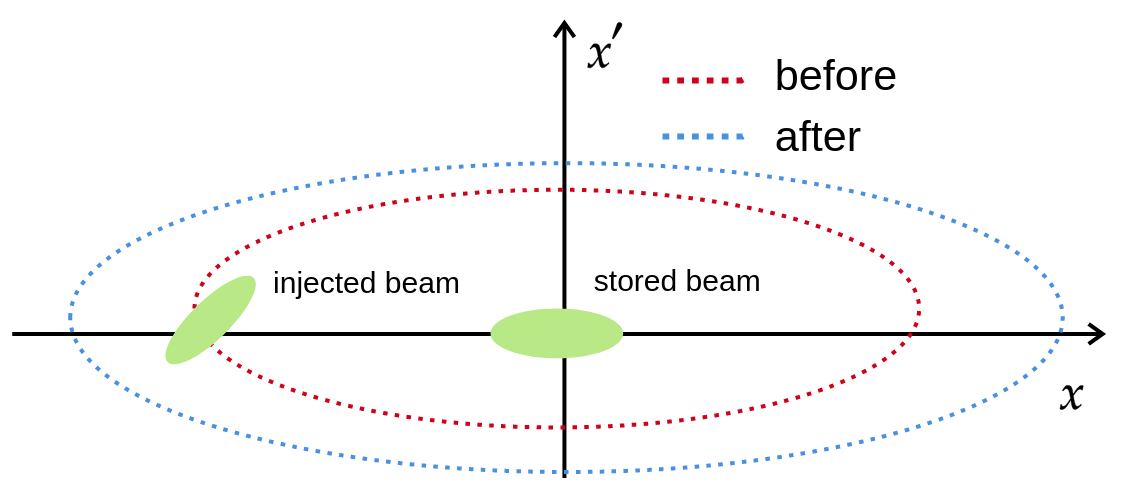
\includegraphics[width=0.7\textwidth]{Images/injection_illustration.png}
    \caption[Illustration of injection sensitivity to the DA]{Illustration of injection sensitivity to the DA. In red, the DA border before optimizing sextupoles. In blue, the expected effect on the DA border after optimization. Reduced injection efficiency results from losing part of the beam due to small DA. Optimizing injection efficiency by tuning sextupoles should translate to optimizing DA.}
    \label{fig:injection_efficiency}
\end{figure}

For online optimization one must choose a practical, relatively fast to measure objective function to act as a probe of the DA: a figure of merit related to the DA to represent it and to be used to evaluate the quality of the changes performed during the online tuning process. In our experiments, we studied using two practical objectives as the probes for DA: the \textbf{injection efficiency} and the \textbf{beam's resilience to dipolar perturbations}. The former is quite self-explanatory: the larger the DA, larger the space for the beam to be captured into the storage ring during the injection pulse, and thus the larger the injection efficiency.

Figure~\ref{fig:injection_efficiency}  illustrates how a smaller aperture, shown in red, influences the efficiency of injection. After leaving the booster accelerator at $3~\unit{GeV}$, the beam is transported into the storage ring injection straight section. It reaches the injection area with phase space coordinates of approximately $(x, x^\prime)\approx(-8~\unit{mm}, 3~\unit{m rad})$. The beam then suffers the deflection of a nonlinear pulsed magnet, the nonlinear kicker (NLK) and is captured into the storage ring with phase space coordinates $(-8~ \unit{mm}, 0)$ \cite{liu_injection_2016}. If the DA border along the negative horizontal direction is reduced below $-8~\unit{mm}$, the dynamics may not accommodate the long term time evolution of the beam fraction exceeding this threshold. This fraction is lost due to the nonlinear dynamics instabilities in the first turns. On the other hand, if the DA is increased, the larger the beam fraction which is successfully captured and survives in the storage ring in the long term.

As for the beam kick resilience, this figure of merit is related to the DA by the following reasoning: the larger the horizontal dipolar kicks the beam can survive, the larger the orbit distortions towards the positive or negative horizontal direction (depending on the kick direction). So the larger the amplitudes the beam explores as it oscillates. If the beam survives to larger kicks, it means the ring can accommodate larger orbit distortions because of an increased DA.

Figure~\ref{fig:action_jump} illustrates the phase space orbits for a beam when it is kicked. In the left sketch, small amplitude TbT motion ellipse is shown. When kicked, the beam gains momentum (angle) and is rigidly translated higher along the $x^{\prime}$ direction. In the linear approximation the beam goes from one ellipse, with action $J$ to another ellipse, with action $\tilde{J}>J$. If the kick is stronger (larger than $500~\unit{\mu rad}$), the action jump takes the beam to a nonlinear regime, as shown in the right sketch, where the beam traces out distorted ellipses. After the kick, the maximum amplitude reached in the negative horizontal direction is increased thus the larger the fraction of the beam that can survive the kick, the larger the DA.

\begin{figure}
    \centering
    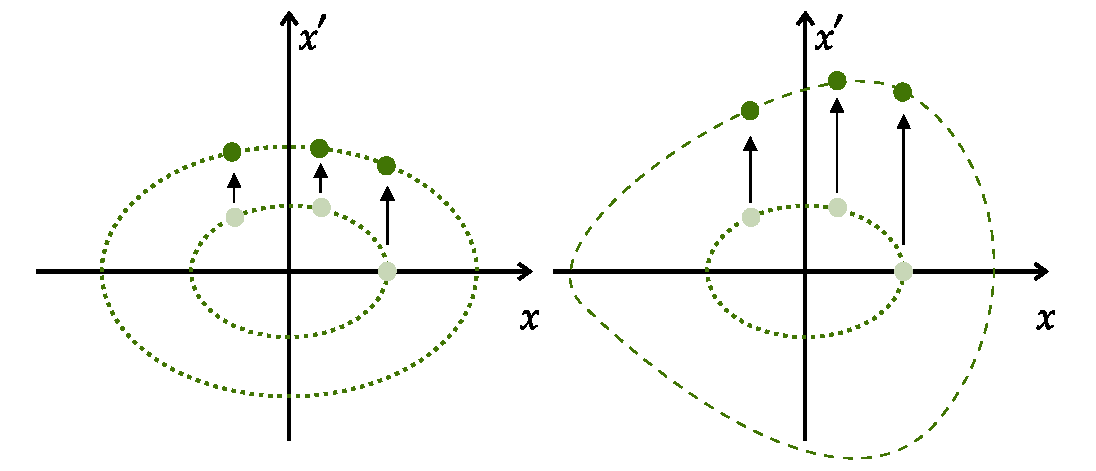
\includegraphics[width=\textwidth]{Images/phase_space_kick.pdf}
    \caption[Action jumps due to dipolar kicks in the linear and nonlinear regimes.]{Action jumps due to dipolar kicks in the linear (left) and nonlinear (right) regimes.}
    \label{fig:action_jump}
\end{figure}

% \subsection{Injection scheme for acummulation at SIRIUS storage ring}
% Beam acummulation into the storage ring occurs in the off-axis scheme. The beam is delivered at $x\approx-8~\unit{mm}$, and receives the kick from the nonlinear kicker field. The field profile is nonlinear, with zero field and gradient at the center of the axis, so that it does not disturbs the stored beam.
% In the off-axis scheme, a sufficiently large dynamic aperture is desired to allow the beam to be captured into the storage ring. The predicted efficiency for SIRIUS setup, considering a dynamic aperture reaching $x=-9~\unit{mm}$, was nearly $100\%$. What was observed during 2022 was an injection efficiency of about $88\pm8\%$.

In summary, the dynamic aperture optimization procedure must consist on the exploration of sextupole (knobs) configurations yielding the largest dynamic aperture as accessed by as objective function such as injection efficiency or beam kick-resiliency.

\subsection{The optimization knobs}
\label{subsec:knobs}
The DA is determined by the quality of the beam dynamics in terms of perturbations. Given that a linear optics correction scheme is already in place and regularly implemented in the machine, effectively addressing optics functions and phase advances, the primary factor impacting SIRIUS DA likely stems from nonlinear dynamics and/or remaining uncorrected and previously inaccessible deviations and errors. This may include sextupole field errors or other minor nonlinear multipoles.

If the limitation of the DA is likely associated with nonlinear dynamics, the actuation knobs must unexpectedly be composed of the controllable nonlinear magnets available at the SIRIUS storage ring, namely the sextupoles. However, it is important to note that sextupole strengths cannot be changed arbitrarily.

Sextupoles are originally introduced into the lattices as actuators for correcting chromaticity, which refers to the energy-dependent aberrations in the focusing of the beam. Care must be taken when varying the sextupole strengths, as it can alter the chromaticity.

A strategy needs to be devised to select the sextupole family in a way that allows for the simultaneous correction of chromaticity and the online tuning of magnet strengths to optimize the DA. In simpler terms, the optimization processes for DA should be conducted while preserving the machine's chromaticity. The natural question that arises is how to implement these isochromatic changes to the sextupoles.

As highlighted previously, SIRIUS has 21 sextupole families, magnets powered by the same power supply. Six of them are achromatic families, strategically placed where the dispersion is zero, while the remaining 15 families are chromatic families. In principle, the optimization parameter space is 21-dimensional. However, as mentioned earlier, the goal is to change sextupoles without affecting chromaticity. Since we need at least one degree of freedom for correcting chromaticity in the horizontal plane and one degree of freedom for correcting chromaticity in the vertical plane, there are 19 independent knobs available. The dimensionality of the search space can be further reduced by imposing additional constraints on certain families' variations. These specific constraints changed according to each experiment and are detailed in what follows. Two strategies were adopted to select the sextupole optimization knobs: a compensation scheme and using the Jacobian null space knobs.

\subsubsection{Compensation scheme}
\label{subsubsec:compensation}
The idea is the following: out of the 15 chromatic sextupole families, at least two of them are labeled "correction" or "compensation" families and are not freely varied by the optimization routine during the experiment. The other 13 chromatic families can be varied arbitrarily, respecting their linear magnetic (non-saturated) regime. Alongside these 13 chromatic families, the strength of the 6 achromatic sextupole families are also free knobs.  Whenever the routine proposes changes in the free knobs, the chromaticity changes caused by this action are anticipated as follows: the reduced Jacobian, $\tilde{\vb{J}}_\xi$, whose columns contain only those corresponding to the free knobs, is used to calculate the chromaticity change $\Delta \boldsymbol{\xi}=\tilde{\vb{J}}_\xi\Delta\vb{S}_{\text{free}}$ upon the change $\Delta\vb{S}_{\text{free}}$ in the free knobs. Another reduced Jacobian, $\vb{J}_{\xi}^{\prime}$ containing only the columns corresponding to the "correction" or "compensation" families is used to counteract the predicted chromaticity build-up, i.e., to produce sextupole changes $\Delta\vb{S}_{\text{corr.}}$ leading to exactly the opposite chromaticity change $-\Delta \boldsymbol{\xi}$. The required strength changes in the compensation families is determined by $\Delta \vb{S}_{\text{corr.}} = \vb{J}_{\xi}^{\prime +}(-\Delta \boldsymbol{\xi}$). Applying $\Delta \vb{S} = \Delta \vb{S}_{\text{free.}} + \Delta \vb{S}_{\text{corr.}}$ to the machine leads to sextupole families strength changes keeping the chromaticity unchanged. The scheme is illustrated in Fig.~\ref{fig:compensation}.

In practice, during the experiments, the compensation scheme was used as follows. The 6 achromatic families plus the SDA1, SFA1, SDB1, SDP1, SDA3, SDB3 and SDP3 families could be freely varied. Their strengths were the optimization knobs. The SDA2, SDB2, SDP2, SFA2, SFB2 and SFP2 were used as the compensation or correction families. They would only be varied to cancel the chromaticity build-up caused by changing the free knobs. The resulting search space was 13-dimensional.

 Note that families SFP1 and SFB1 were not used as knobs. They were kept constant. They were actually used in the first experiments attempts, as discussed in section~\ref{sec:kick_res_opt} of the next chapter, but were later removed upon the realization that they already operate close to saturation, where the fields may not be repeatable due to hysteresis effect. When these are included, the search space is 15-dimensional.

 The compensation families were chosen on basis of having range to act on the chromaticity, that is, they were the families with initial strengths far from saturation, with a lot of room to compensate the knobs effects on chromaticity.
\begin{figure}
    \centering
    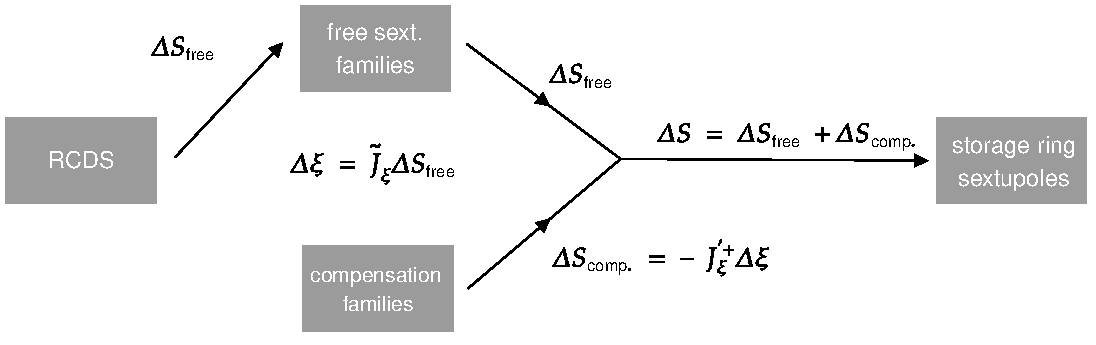
\includegraphics[width=\textwidth]{Images/compensation_scheme.pdf}
    \caption[Illustration of the compensation scheme for changing sextupole strengths with no change in chromaticity.]{Illustration of the compensation scheme for changing sextupole strengths with no change in chromaticity.}
    \label{fig:compensation}
\end{figure}
\subsubsection{Jacobian null space knobs scheme}
\label{subsubsec:nullspace}
Here the idea is to identify the combination of sextupole families living in the null space, or kernel, of the chromaticity Jacobian matrix. That is, we are interested in the set of vectors $\text{ker}(\vb{J}_\xi)=\text{span}\{\vb{s}_i\in\mathbb{R}^{21}| \vb{J}_{\xi} \vb{s}_i = \vb{0}\}_{i=1,\dots,19}$. If we perform changes along such subspace $\Delta \vb{S}\in\text{ker}(\vb{J}_\xi)$ then the resulting changes in chromaticity are null.

The reason why we can anticipate the dimension of the null space is 19 is because it contains the 6 achromatic sextupole families plus 13 degrees of freedom out of the 15 achromatic families, since at least 2 degrees of freedom are needed to act over chromaticity.

A straightforward way to identify the null space of the Jacobian is to calculate its full singular value decomposition (SVD), which expresses the Jacobian as the product
\begin{equation}
    \begin{aligned}
        \vb{J}_\xi &= \vb{U}\boldsymbol{\Sigma}\vb{V}^\intercal\\
                   &= \underbrace{\mqty[\vdots & \vdots \\
                            \vb{u}_1 & \vb{u}_2\\
                            \vdots & \vdots]}_{2\times 2}
                            \underbrace{\mqty[\sigma_1 & 0 & \dots & 0\\
                                             0 & \sigma_2 & \dots & 0 ]}_{2\times21}
                            \underbrace{\mqty[
                                \dots & \vb{v}^\intercal_1 & \dots\\
                                \dots & \vb{v}^\intercal_2 & \dots\\
                                \dots & \vb{v}^\intercal_3 & \dots\\
                                      & \vdots &    \\
                                \dots & \vb{v}^\intercal_{21} & \dots\\                              ]}_{21\times21}.
    \end{aligned}
\end{equation}
Note that the singular-values matrix has only two non-vanishing singular values $\sigma_1$ and $\sigma_2$. In the sum-over-modes form of SVD, we have
\begin{equation}
    \vb{J}_\xi = \sum_{i=0}^{21}\sigma_i\vb{u}_i\vb{v}_{i}^{\intercal} = \sigma_1 \vb{u}_1\vb{v}_{1}^\intercal + \sigma_2 \vb{u}_2\vb{v}_{2}^\intercal,
\end{equation}
in which it becomes clear that we have only two independent modes or degrees of freedom for changing chromaticity, corresponding to the horizontal and vertical degrees of freedom.

Multiplication of the SVD-decomposed $\vb{J}_{\xi}$ by $\vb{V}$ gives $\vb{J}_{\xi}\vb{V} = \vb{U}\boldsymbol{\Sigma}$, which explicitly reads
\begin{equation}
    \begin{aligned}
        \vb{J}_{\xi}\vb{v}_i & = \sigma_i \vb{u}_i, \quad i=1,2,\\
        \vb{J}_{\xi}\vb{v}_i & = \vb{0}, \quad i=3,\dots,21.\\
    \end{aligned}
\end{equation}
Revealing the sextupole strength vectors living in the null space of the Jacobian. They must be the ones associated with the vanishing singular values: $\text{ker}(\vb{J}_\xi) = \text{span}\{\vb{v}_i\}_{i=3,\dots,21}$.
%  Referring to our previous notation, we can say $\text{ker}(\vb{J}_\xi) = \text{span}\{\vb{s}_i = \vb{v}_{i+2}\}_{i=1,\dots,19}$.
Figure~\ref{fig:chrom_jac_subspaces} illustrates the fundamental subspaces associated with the chromaticity jacobian. The range of the matrix, or column space, is the chromaticity changes space. Vectors living in the null space are the sextupole strengths combinations mapped to the chromaticity space origin.

\begin{figure}
    \centering
    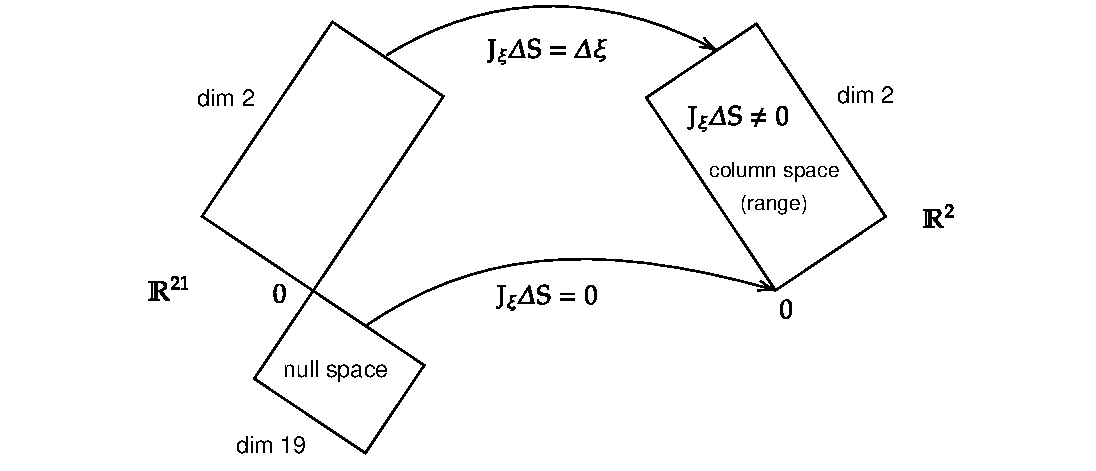
\includegraphics[width=0.8\textwidth]{Images/chrom_jacobian_subspaces.pdf}
    \caption[Illustration of chromaticity jacobian $\vb{J}_{\xi}$ fundamental subspaces]{Illustration of chromaticity jacobian $\vb{J}_{\xi}$ fundamental subspaces. The idea is to use sextupole combinations living in the null space, since these are mapped to the zero vector on the chromaticity space.}
    \label{fig:chrom_jac_subspaces}
\end{figure}

As mentioned previously, additional constraints on the families strengths variations  have been imposed to further reduce the dimensionality of the search space. In such cases, the jacobian is recalculated considering the imposed constraints. For instance, in one of the experiments the following constraints were imposed:
\begin{itemize}
    \item Families SFP1 and SFB1 were kept constant, i.e., were not allowed to change. As mentioned, they operate close to their saturation, nonlinear regime, and one cannot trust they would be able to provide reproducible magnetic field changes. Deciding not using them already reduces from 21 to 19 degrees of freedom.
    \item The pair of families SDB1 \& SDP1, SDB2 \& SDP2, SFB2 \& SFP2, SDB3 \& SDP3 were constrained to change by the same amount, starting from their respective initial strengths. This reduces the available options from 19 to 15 families.
\end{itemize}
These 15 families consist on the combination of the 6 achromatic families, the 4 pairs of constrained families and 5 other non-constrained families SDA1, SFA1, SDA2 , SFA2, and SDA3.
% The 9-dimensional chromatic space Jacobian is calculated and its null space basis reveals the 7-dimensional space spanned by the linear combination of sextupole strengths that will not change chromaticity when varied. Combining the 7-dimensional null space with achromatic families results in a 13-dimensional search space. We shall refer to such constraint configuration as \textbf{Constraint Scheme I}, to distinguish it from \textbf{Constraints Scheme II}, which consists on
Calculating the null space of the Jacobian results in a 13-dimensional search space. We shall refer to such constraint configuration as \textbf{Constraint Scheme I}, to distinguish it from \textbf{Constraint Scheme II}, which consists on

\begin{itemize}
    \item Families SFP1 and SFB1 were kept constant, by the same reason as in the previous scheme.
    \item No pair-wise constraints were imposed to the sextupole families. So, in principle, there were 19 possible families: 21 minus the two families not used.
\end{itemize}
Calculating the Jacobian null space revealed the 17 chromaticity-preserving free knobs.

% With the presentation of experimental procedures, setup and the available diagnostics, we can move on to reporting the experiments and their results. This is the focus of the next chapter.
% \subsection{Characterization of Sextupole Magnets Configurations}
% Once a configuration of sextupoles (position in parameter space) is found, the nonlinear optics it provides the machine needs to be characterized. The characterizations consisted on evaluatig/measuring the followint figures of merit and desired features
% \begin{itemize}
%     \item Injection efficiency in nominal off-axis conditions : this is the most desired characteristic. The sextupoles are to be optimized so the DA and the off-axis injection efficiency increase.
%     \item Beam Kick resilience: a small current of $2~\unit{\milli\ampere}$, concentrated in a single bucket is stored in the ring. The beam is kicked by the horizontal dipole kicker, which instantly provides a dipolar perturbation leading the beam to be displaced in the horizontal direction. The current before and after the kick is recorded by a current monitor (DCCT) and allows for the calculation of the fraction of the beam lost as a consequence of the kick and the transverse displacement. The procedure is repeated with progressively stronger kicks, and a curve of beam loss as a function of the kick can be constructed. The smaller the losses for larger kicks, the larger the resilience.
%     \item Phase portrait area: it is expected that the optimzation procedure increases the dynamic aperture of the machine, meaning it can accomodate larger oscillations and larger phase portraits $x-x^\prime$. Using beam position monitors (BPMs) at the two ends of a straight section, which record the positions of the beam centroid at each turn, we can calculate the position and angle of the beam in the middle of the straight section, and thus recostruct the phase-portrait from turn-by-turn (TbT) data.
%     \item Beam lifetime: the lifetime at SIRIUS is dominated by losses due to electron-electron interactions leading to momentum transfers exceeding the energy/momentum acceptance (MA). Optimization of DA does not necessarily leads to improvements in the MA. If the MA is reduced, the rate at which the beam is lost can increase, reducing the total lifetime. It is desireble that the configurations found during DA otpimzation do not worsen the MA and beam lifetime considerably.
%     % One dominat effect leading to beam loss is the so-called Touschek Effect, consisiting on collisions between electrons of the same bunch leading to momentum trasfers from the transverse to the longitudinal direction that can exceed the lattice tolerance to momentum deviations, the Momentum Acceptance. Momentum acceptance is the dynamic aperture for off-energy particles. Optimization of DA, which is accesed by the aforementioned objective functions, not necessarily leads to improvements in the MA. If the MA is reduced, the rate of Touschek events increases and thus the lifetime is reduced. Therefore, another desired feature from a good sextupole configurations is having a good beam lifetime. We expect not the worsen the lifetime.
%     \item Chromaticity: Sextupoles are introduced in the storage ring for correction of focusing chromatic aberretions. When changing the sextupole settings, it is desired to do so in such a manner that the chromaticity is unchanged. The methods for choosing the optimization knobs already take into account the need for keeping constant chromaticity. Still, after optimization is performed, we need to check whether chromaticity is unchanged.
% \end{itemize}
% The first two characterizations are quite similar to the two most immediate objective function candidates mentioned above. Indeed, in most nonlinear dynamics optimzation experiments, optimization using injection efficiency or kick resilience as objectives seemed to be completely interchangable. Improvements in injection efficiency necessarily led to improvements in kick resilience, and vice-versa. As shown in more details in the results section, for the SIRIUS storage ring this appears not to be the case. The configurations can be specialized to improvements solely on injection efficiency or solely to kick resilience. This feature was observed during the characterization of the optimized sextupole settings with respect to these two figures of merit.
